% ============================================================
%  midsub_v4.tex -- EVS Project #19 Mid-Evaluation (version 4)
%  Based on midsub_v3.tex (concise) with team feedback:
%  numeric citations, GPP / carbon-sink slide, v2 text for methods and
%  results, workflow-first methodology, clearer response surface.
%  Compile (from slides/): pdflatex midsub_v4; bibtex midsub_v4;
%                          pdflatex midsub_v4; pdflatex midsub_v4
%  Numbers: same sources as the other versions (see NUMBERS.md).
%  New figure: python slides/make_v4_figures.py
% ============================================================
\documentclass[11pt,aspectratio=169]{beamer}

\usetheme{Madrid}
\usecolortheme{seahorse}

\usepackage[T1]{fontenc}
\usepackage[utf8]{inputenc}
\usepackage{tikz}
\usetikzlibrary{positioning, arrows.meta}
\usepackage{booktabs}
\usepackage{graphicx}
\usepackage{multirow}
\usepackage{array}
\newcolumntype{L}[1]{>{\raggedright\arraybackslash}p{#1}}
% natbib's [numbers] package option breaks this TinyTeX install (missing
% grfext.sty), so numeric citations are switched on with \setcitestyle instead
\usepackage{natbib}
\setcitestyle{numbers,square,comma,sort&compress}
\bibliographystyle{unsrtnat}
\setbeamertemplate{bibliography item}{\insertbiblabel}

\newcommand{\FigPath}[1]{../figures/#1.png}
\newcommand{\Fig}[2]{\includegraphics[width=#2,height=0.66\textheight,keepaspectratio]{\FigPath{#1}}}

\title[Compound Heat-Drought Stress]{Compound Heat--Drought Stress over India}
\subtitle{Are ecosystems hit harder when heat and drought strike together?\\[2pt]
  \small Mid-Evaluation, EVS Project \#19}
\author[EVS Project \#19]{
  Arnav Deshmukh \and Ayush Brajesh Roy \and Saksham Chitkara \and
  Gracy Garg \and Rudra Choudhary
}
\institute{IIIT Hyderabad}
\date{\today}

\begin{document}

\frame{\titlepage}

\begin{frame}{Outline}
  \tableofcontents
\end{frame}

% =================================================================
\section{Problem statement \& motivation}
% =================================================================

\begin{frame}{Heat and drought rarely come alone}
  \begin{columns}
    \column{0.36\linewidth}
    \small
    \begin{itemize}
      \item \textbf{Drought}: too little water (little rain, dry soil)
      \item \textbf{Heat}: high temperature, ``thirsty'' air
      \item They feed each other: dry soil heats up, heat dries soil
      \item Plants get hit from both sides
    \end{itemize}
    \column{0.62\linewidth}
    \centering
    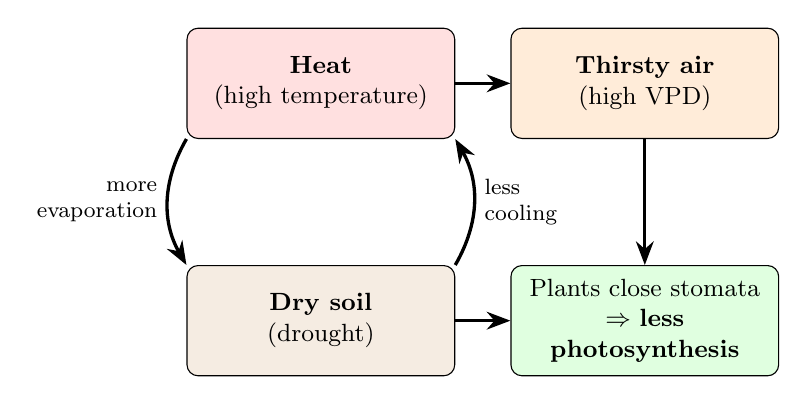
\begin{tikzpicture}[
        node distance=16mm and 7mm,
        b/.style={draw, rounded corners, align=center, font=\small,
                  minimum width=3.4cm, minimum height=1.4cm},
        a/.style={-{Stealth[length=3mm]}, very thick}]
      \node[b, fill=red!12] (heat) {\textbf{Heat}\\(high temperature)};
      \node[b, fill=orange!15, right=of heat] (vpd) {\textbf{Thirsty air}\\(high VPD)};
      \node[b, fill=brown!15, below=of heat] (soil) {\textbf{Dry soil}\\(drought)};
      \node[b, fill=green!12, below=of vpd] (gpp) {Plants close stomata\\$\Rightarrow$ \textbf{less}\\\textbf{photosynthesis}};
      \draw[a] (heat) -- (vpd);
      \draw[a] (vpd) -- (gpp);
      \draw[a] (soil) -- (gpp);
      \draw[a] (heat.south west) to[bend right=30] node[left, font=\footnotesize, align=right]{more\\evaporation} (soil.north west);
      \draw[a] (soil.north east) to[bend right=30] node[right, font=\footnotesize, align=left]{less\\cooling} (heat.south east);
    \end{tikzpicture}
  \end{columns}
\end{frame}

\begin{frame}{Key idea: GPP and the land carbon sink}
  \small
  \textbf{Gross primary productivity (GPP)} is the total amount of carbon that
  plants take out of the air by photosynthesis, per area and time (we use grams
  of carbon per m$^2$ per month). It is the starting point of plant growth, crop
  yield and the land carbon sink.

  \vspace{4pt}
  \centering
  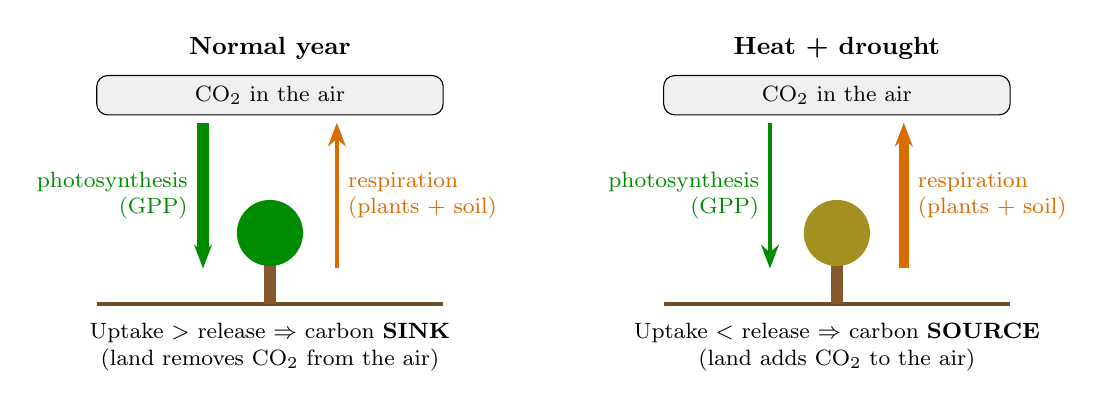
\begin{tikzpicture}[font=\footnotesize]
    \foreach \x/\ttl/\gw/\rw/\crown/\verdict in {
        0/Normal year/4.5pt/1.5pt/green!55!black/{Uptake $>$ release $\Rightarrow$ carbon \textbf{SINK}\\(land removes CO$_2$ from the air)},
        7.2/Heat + drought/1.2pt/3.5pt/olive!60!brown/{Uptake $<$ release $\Rightarrow$ carbon \textbf{SOURCE}\\(land adds CO$_2$ to the air)}} {
      \begin{scope}[xshift=\x cm]
        \node[font=\small\bfseries] at (0,3.25) {\ttl};
        \node[draw, rounded corners, fill=gray!12, minimum width=4.4cm, minimum height=0.5cm] at (0,2.65) {CO$_2$ in the air};
        \draw[very thick, brown!60!black] (-2.2,0) -- (2.2,0);
        \fill[brown!70!black] (-0.08,0) rectangle (0.08,0.55);
        \fill[\crown] (0,0.9) circle (0.42);
        \draw[-{Stealth[length=3mm]}, line width=\gw, green!55!black] (-0.85,2.3) -- (-0.85,0.45)
          node[midway, left, align=right] {photosynthesis\\(GPP)};
        \draw[-{Stealth[length=3mm]}, line width=\rw, orange!85!black] (0.85,0.45) -- (0.85,2.3)
          node[midway, right, align=left] {respiration\\(plants + soil)};
        \node[align=center] at (0,-0.55) {\verdict};
      \end{scope}
    }
  \end{tikzpicture}

  \vspace{2pt}
  \footnotesize Heat + drought can flip land from sink to source: Europe in 2003
  \citep{ciais2005}.
\end{frame}

\begin{frame}{Why it matters}
  \begin{itemize}
    \item \textbf{Europe 2003}: a summer of heat + drought cut productivity by
      about 30\% and turned Europe's land into a temporary carbon
      \emph{source} \citep{ciais2005}.
    \item \textbf{Worldwide}: across flux-tower sites, combined heat + drought
      reduced the carbon sink more than either extreme alone
      \citep{vonbuttlar2018}.
    \item \textbf{India}: droughts and heatwaves that happen at the same time
      have become more frequent and widespread \citep{sharma2017}.
    \item As the climate warms, more droughts will happen during hot spells,
      so we need to know how much worse the combination is.
  \end{itemize}
\end{frame}

\begin{frame}{Why India?}
  \begin{columns}
    \column{0.56\linewidth}
    \small
    \begin{itemize}
      \setlength{\itemsep}{6pt}
      \item \textbf{Monsoon-dependent}: most rain falls in Jun--Sep; a weak
        monsoon means drought (2002, 2009).
      \item \textbf{Hot pre-monsoon}: Mar--May is the hottest season; extreme
        heat in 2010 and 2022.
      \item \textbf{Mostly cropland} ($\sim$60\% of cells): lost productivity
        means lost food and income.
      \item \textbf{Under-studied}: most work covers Europe, China or the
        globe; India-wide studies are new \citep{meena2026,sen2026}.
    \end{itemize}
    \column{0.44\linewidth}
    \centering
    \includegraphics[width=\linewidth,height=0.8\textheight,keepaspectratio]{\FigPath{study_area_landcover}}
  \end{columns}
\end{frame}

\begin{frame}{Problem statement}
  \centering
  \Large
  \textbf{Topic \#19: Compound Heat--Drought Stress}\\[4pt]
  \large Are ecosystems experiencing stronger combined impacts?

  \vspace{14pt}
  \normalsize
  Does simultaneous heat and drought produce \textbf{greater ecosystem stress}
  than either disturbance alone?

  \vspace{16pt}
  \begin{block}{Why this matters}
    \large
    If heat and drought damage simply \textbf{add up}, we can predict compound
    impacts from single-stress studies. If they \textbf{amplify} each other,
    compound events are a separate, bigger risk.
  \end{block}
\end{frame}

\begin{frame}{Our questions (for India)}
  \begin{enumerate}
    \setlength{\itemsep}{8pt}
    \item Is vegetation hit harder in \textbf{compound} (hot \emph{and} dry)
      months than in hot-only or dry-only months?
    \item Is the compound hit \textbf{bigger than the heat damage plus the
      drought damage added together}?
    \item Do ecosystems take \textbf{longer to recover} after compound events?
    \item Does the answer differ between \textbf{forests, croplands,
      grasslands}, and between \textbf{Peninsular and North India}?
  \end{enumerate}
\end{frame}

\begin{frame}{What is known, and what is still open}
  \footnotesize
  \begin{columns}[T]
    \column{0.48\linewidth}
    \textbf{\normalsize Known}
    \begin{itemize}
      \setlength{\itemsep}{4pt}
      \item Heat + drought together cut the carbon uptake of ecosystems more
        than either extreme alone (flux towers worldwide
        \citep{vonbuttlar2018}; Europe 2003 \citep{ciais2005}).
      \item In India, hot and dry conditions together raise the
        \emph{chance} that vegetation goes into drought \citep{meena2026}.
      \item In Peninsular India's forests, compound hot--dry extremes raise the
        risk of large GPP losses \citep{sen2026}.
    \end{itemize}
    \column{0.5\linewidth}
    \textbf{\normalsize Open}
    \begin{itemize}
      \setlength{\itemsep}{4pt}
      \item Is the damage to \emph{average} productivity more than heat damage
        + drought damage (synergy), or just the sum? Few studies test this
        directly, with uncertainty.
      \item The answer depends on how ``drought'' is defined: soil-based and
        air-based definitions give different impacts \citep{liang2026}.
      \item Do ecosystems recover more slowly after compound events? Global
        studies disagree \citep{yao2024,huang2025,feng2026}, and we found no
        India-specific comparison.
    \end{itemize}
  \end{columns}
\end{frame}

% =================================================================
\section{Our hypotheses}
% =================================================================

\begin{frame}{Our hypotheses}
  \small
  \textbf{Our aim:} an India-wide, honest test of additivity on two satellite
  measures, with uncertainty and a drought-index check, then recovery and
  regional differences. This is a regional synthesis with extensions, not a
  first-of-its-kind study.

  \vspace{6pt}
  \renewcommand{\arraystretch}{1.15}
  \begin{tabular}{@{}L{0.07\linewidth}L{0.66\linewidth}L{0.22\linewidth}@{}}
    \toprule
    & \textbf{Hypothesis} & \textbf{Current status} \\
    \midrule
    \textbf{H1} & Vegetation (GPP, NDVI) is lower in compound months than in
      hot-only or dry-only months. & \textbf{Tested} \\
    \textbf{H2} & The compound effect is \emph{synergistic}: larger than the
      heat effect + the drought effect. & \textbf{Tested} \\
    \textbf{H3} & Ecosystems recover more slowly after compound events than
      after droughts. & In progress \\
    \textbf{H4} & The response differs by land cover and by region
      (Peninsular vs North India). & In progress \\
    \bottomrule
  \end{tabular}

  \vspace{6pt}
  \scriptsize Throughout, we check that conclusions do not depend on the
  choice of drought index (SPEI-3 vs SPI-3).
\end{frame}

% =================================================================
\section{Methodology}
% =================================================================

\begin{frame}{Workflow}
  \centering
  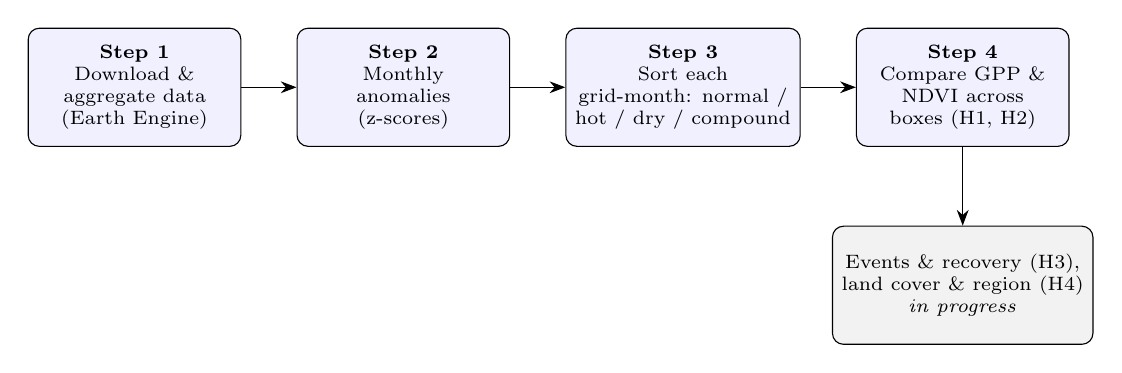
\begin{tikzpicture}[
      node distance=7mm,
      box/.style={draw, rounded corners, align=center, minimum width=2.7cm,
                  minimum height=1.5cm, font=\scriptsize, fill=blue!6},
      arr/.style={-{Stealth[length=2mm]}}]
    \node[box] (a) {\textbf{Step 1}\\Download \&\\aggregate data\\(Earth Engine)};
    \node[box, right=of a] (b) {\textbf{Step 2}\\Monthly\\anomalies\\(z-scores)};
    \node[box, right=of b] (c) {\textbf{Step 3}\\Sort each\\grid-month: normal /\\hot / dry / compound};
    \node[box, right=of c] (d) {\textbf{Step 4}\\Compare GPP \&\\NDVI across\\boxes (H1, H2)};
    \node[box, below=10mm of d, fill=gray!10] (e) {Events \& recovery (H3),\\land cover \& region (H4)\\\textit{in progress}};
    \draw[arr] (a) -- (b); \draw[arr] (b) -- (c); \draw[arr] (c) -- (d); \draw[arr] (d) -- (e);
  \end{tikzpicture}

  \vspace{10pt}
  \footnotesize Everything is scripted in Python (xarray, scipy, statsmodels)
  and checked by 68 automated tests. The analysis reruns from cached data in
  minutes.
\end{frame}

\begin{frame}{Step 1: data}
  \scriptsize
  \renewcommand{\arraystretch}{0.95}
  \begin{tabular}{@{}L{0.21\linewidth}L{0.33\linewidth}L{0.12\linewidth}L{0.27\linewidth}@{}}
    \toprule
    \textbf{Dataset} & \textbf{What we use} & \textbf{Period} & \textbf{Role} \\
    \midrule
    ERA5-Land \citep{munozsabater2021} & daily max temperature; soil moisture 0--100 cm; VPD & 1991--2024 & defines ``hot''; mechanism \\
    SPEI v2.11 \citep{vicenteserrano2010} & SPEI-3 (rain minus evaporative demand) & 1991--2024 & defines ``dry'' \\
    CHIRPS v2 \citep{funk2015} & rainfall $\rightarrow$ SPI-3 & 1991--2024 & temperature-free drought check \\
    MODIS MOD17A2H \citep{running2015,running2004} & GPP (photosynthesis) & 2001--2022 & main response \\
    MODIS MOD13A3 \citep{didan2021} & NDVI (greenness), quality-masked & 2001--2022 & second response \\
    ESA WorldCover \citep{zanaga2022} & land-cover fractions & 2021 & vegetation mask; land-cover groups \\
    \bottomrule
  \end{tabular}

  \vspace{6pt}
  \begin{itemize}
    \item All five suggested datasets, processed in Google Earth Engine
      \citep{gorelick2017} onto one common grid: 0.25\textdegree{} ($\approx$27 km),
      monthly, all of India (4,481 grid cells).
    \item GPP and NDVI both come from the MODIS Terra satellite: two
      different products, but not independent sensors.
  \end{itemize}
\end{frame}

\begin{frame}{Metrics at a glance}
  \scriptsize
  \renewcommand{\arraystretch}{1.0}
  \begin{tabular}{@{}L{0.14\linewidth}L{0.53\linewidth}L{0.27\linewidth}@{}}
    \toprule
    \textbf{Metric} & \textbf{What it measures} & \textbf{How to read it} \\
    \midrule
    \multicolumn{3}{@{}l}{\textit{Ecosystem response}} \\
    GPP & Carbon taken up by plants through photosynthesis (gC/m$^2$/month) & higher = more productive \\
    NDVI & Canopy greenness from red and near-infrared reflectance (0--1) & higher = greener \\
    \midrule
    \multicolumn{3}{@{}l}{\textit{Stress}} \\
    Tmax $z$ & Anomaly of the monthly mean daily maximum temperature & $\ge 1$: ``hot'' month \\
    SPEI-3 & 3-month water balance: rain minus evaporative demand & $\le -1$: ``dry'' month \\
    SPI-3 & 3-month rainfall only (no temperature in it) & $\le -1$: dry (robustness) \\
    Soil moisture & Water in the top 1 m of soil & lower = drier soil \\
    VPD & Vapour-pressure deficit: how ``thirsty'' the air is & higher = more water stress \\
    \midrule
    \multicolumn{3}{@{}l}{\textit{Statistics}} \\
    $z$-score & Distance from normal for that place and calendar month (in SDs) & 0 = normal; $-1$ = clearly low \\
    Amplification & Compound effect $-$ (heat effect + drought effect) & $<0$ synergy; $\approx0$ additive \\
    95\% CI & Year-block bootstrap: 1,000 resamples of whole years & excludes 0 = significant \\
    \bottomrule
  \end{tabular}
\end{frame}

\begin{frame}{Step 2: monthly anomalies (comparing like with like)}
  \small
  \begin{itemize}
    \item Raw values are not comparable: May is always hotter than January,
      and a desert always has less GPP than a forest.
    \item So for every grid cell and every calendar month, we convert a value
      into a \textbf{z-score}:
      \[
        z = \frac{\text{this month's value} - \text{normal for this cell in this month}}
                 {\text{typical year-to-year spread}}
      \]
      $z = -1$ means ``one standard deviation below what is normal here at
      this time of year''.
    \item \textbf{Temperature}: normal = 1991--2020. Not detrended, so
      long-term warming counts as heat.
    \item \textbf{GPP, NDVI}: a linear trend is removed first, so the
      long-term greening of India (CO$_2$, irrigation) is not mistaken for
      an anomaly.
    \item \textbf{Only growing-season months count}: the cell is in India,
      at least 50\% vegetated, and GPP in that month is normally at least
      30\% of its peak. This removes deserts and dormant seasons
      (824,598 grid-months remain).
  \end{itemize}
\end{frame}

\begin{frame}{Step 3: sorting every grid-month into four boxes}
  \begin{columns}
    \column{0.44\linewidth}
    \centering
    \renewcommand{\arraystretch}{1.4}
    \begin{tabular}{cc|c|c}
      & & \multicolumn{2}{c}{SPEI-3 (dryness)} \\
      & & $> -1$ & $\le -1$ \\
      \hline
      \multirow{2}{*}{Tmax $z$} & $< 1$ & Normal & Dry-only \\
      & $\ge 1$ & Hot-only & \textbf{Compound} \\
    \end{tabular}

    \vspace{6pt}
    \scriptsize
    \begin{tabular}{@{}lr@{}}
      Normal & 573,543 \\
      Hot-only & 79,717 \\
      Dry-only & 109,073 \\
      \textbf{Compound} & \textbf{62,265} (7.6\%) \\
    \end{tabular}
    \column{0.54\linewidth}
    \scriptsize
    \begin{itemize}
      \item \textbf{Hot}: the month's average daily maximum temperature is at
        least 1 standard deviation above normal.
      \item \textbf{Dry}: SPEI-3 $\le -1$, i.e.\ the last 3 months had
        clearly less water than usual (rain minus evaporative demand).
      \item SPEI's demand term depends on temperature, so ``dry'' is partly
        driven by heat. We therefore repeat everything with
        \textbf{SPI-3}, which uses rainfall only.
      \item Left: number of growing-season grid-months in each box, India,
        2001--2022.
    \end{itemize}
  \end{columns}
\end{frame}

\begin{frame}{Step 4: how we test H1 and H2}
  \small
  \begin{itemize}
    \item \textbf{H1}: average GPP $z$ (and NDVI $z$) in each box, and the
      differences between boxes.
    \item \textbf{H2}: compare the compound effect with the sum of the single
      effects. Each effect is measured relative to normal months:
      \[
        \text{Amplification} = \Delta_{\text{compound}} -
          \left(\Delta_{\text{hot}} + \Delta_{\text{dry}}\right)
      \]
      \vspace{-10pt}
      \begin{itemize}
        \item $< 0$: compound is worse than the sum $\Rightarrow$ \textbf{synergy};
        \item $\approx 0$: \textbf{additive};
        \item $> 0$: less than the sum (\textbf{sub-additive}).
      \end{itemize}
    \item \textbf{Uncertainty}: 95\% confidence intervals from a
      \emph{year-block bootstrap}. We resample whole years (1,000 times), because
      neighbouring cells in the same year are not independent. A result is
      called significant when its interval excludes zero.
  \end{itemize}
\end{frame}

% =================================================================
\section{Preliminary analysis (H1, H2)}
% =================================================================

\begin{frame}{Where compound months happen}
  \begin{columns}
    \column{0.5\linewidth}
    \centering
    \Fig{freq_map_compound}{\linewidth}
    \column{0.48\linewidth}
    \small
    \begin{itemize}
      \item Share of each cell's growing-season months that were compound,
        2001--2022.
      \item Overall, 7.6\% of growing-season grid-months are compound.
      \item Hotspots: the northern plains, east-central India, the
        North-East, and a belt in the western Deccan (around 15--18\textdegree N).
      \item Both North and Peninsular India have more than 20,000 compound
        grid-months, enough for a reliable comparison.
    \end{itemize}
  \end{columns}
\end{frame}

\begin{frame}{H1: is vegetation hit harder in compound months?}
  \centering
  \Fig{composite_gpp_z_overall}{0.47\linewidth}
  \hfill
  \Fig{composite_ndvi_z_overall}{0.47\linewidth}

  \scriptsize
  \begin{tabular}{@{}lcccc@{}}
    \toprule
    Mean $z$ [95\% CI] & Normal & Hot-only & Dry-only & Compound \\
    \midrule
    GPP  & $+0.12$ & $-0.13$ [$-0.24,-0.01$] & $-0.27$ [$-0.40,-0.15$] & $\mathbf{-0.43}$ [$-0.54,-0.33$] \\
    NDVI & $+0.19$ & $-0.37$ [$-0.50,-0.26$] & $-0.30$ [$-0.41,-0.21$] & $\mathbf{-0.68}$ [$-0.81,-0.55$] \\
    \bottomrule
  \end{tabular}
\end{frame}

\begin{frame}{H1: result}
  \small
  \begin{itemize}
    \item All three stress types lower productivity and greenness
      significantly compared with normal months.
    \item \textbf{Compound months are the worst}, and significantly worse
      than either single stress:
      \begin{itemize}
        \item compound minus dry-only: GPP $-0.16$ [$-0.26,-0.04$],
          NDVI $-0.38$ [$-0.49,-0.28$];
        \item compound minus hot-only: GPP $-0.30$ [$-0.40,-0.21$],
          NDVI $-0.31$ [$-0.43,-0.21$].
      \end{itemize}
    \item Robust to the drought index. With rainfall-only SPI-3, compound
      minus dry-only is GPP $-0.26$ [$-0.37,-0.13$] and NDVI $-0.48$
      [$-0.61,-0.35$].
    \item \textbf{Why?} Compound months combine the driest soils \emph{and}
      the thirstiest air:

      \vspace{2pt}
      \scriptsize
      \begin{tabular}{@{}lcccc@{}}
        \toprule
        & Normal & Hot-only & Dry-only & Compound \\
        \midrule
        Root-zone soil moisture $z$ & $+0.29$ & $-0.75$ & $-0.38$ & $\mathbf{-1.04}$ \\
        Air dryness (VPD) $z$ & $-0.38$ & $+1.11$ & $+0.18$ & $\mathbf{+1.43}$ \\
        \bottomrule
      \end{tabular}
  \end{itemize}
  \vspace{2pt}
  \textbf{H1 supported.}
\end{frame}

\begin{frame}{H2: is the combination worse than the sum?}
  \centering
  \includegraphics[width=0.92\linewidth]{\FigPath{additivity_gpp_ndvi}}

  \scriptsize Hatched bar: what we would expect if the two damages simply
  added up. Green bar: what actually happened in compound months.
\end{frame}

\begin{frame}{H2: result}
  \begin{columns}[T]
    \column{0.5\linewidth}
    \small
    Amplification $= \Delta_{\text{compound}} - (\Delta_{\text{hot}} +
    \Delta_{\text{dry}})$; $<0$ would mean synergy.

    \vspace{6pt}
    \begin{tabular}{@{}lrr@{}}
      \toprule
      & with SPEI-3 & with SPI-3 \\
      \midrule
      GPP  & $+0.09$ & $-0.00$ \\
           & \scriptsize[$-0.03$, $+0.21$] & \scriptsize[$-0.12$, $+0.13$] \\
      NDVI & $+0.18$ & $+0.06$ \\
           & \scriptsize[$+0.06$, $+0.30$] & \scriptsize[$-0.05$, $+0.18$] \\
      \bottomrule
    \end{tabular}
    \column{0.48\linewidth}
    \small
    \begin{itemize}
      \item \textbf{No synergy}: the amplification is never significantly
        negative.
      \item Heat and drought damages roughly \textbf{add up}. Compound
        months are worse than either alone, but not worse than both
        together.
      \item With SPEI-3, NDVI is even slightly \emph{less} than additive,
        but this disappears with SPI-3. The drought definition matters.
    \end{itemize}
  \end{columns}
  \vspace{6pt}
  \small \textbf{H2 not supported} (for average productivity, India-wide).
\end{frame}

\begin{frame}{H2: response surface (a check without boxes)}
  \begin{columns}
    \column{0.48\linewidth}
    \centering
    \includegraphics[width=\linewidth,height=0.8\textheight,keepaspectratio]{\FigPath{response_surface_gpp_explained}}
    \column{0.51\linewidth}
    \footnotesize
    \textbf{What you are looking at}
    \begin{itemize}
      \item x = heat (Tmax $z$); y = water balance (SPEI-3, lower = drier).
      \item Each square: average GPP $z$ of all months in that range
        (red = below normal; grey = fewer than 30 months).
      \item Dashed lines = our cut-offs; bottom-right = the compound box.
    \end{itemize}

    \textbf{What we see}
    \begin{itemize}
      \item GPP falls as it gets drier: about $+0.5$ in the wettest rows,
        $-0.35$ in the driest.
      \item Worst square: hottest + driest corner ($-0.92$). Hot but wet
        months are not below normal.
      \item $\Rightarrow$ Dryness is the main driver and heat adds to it,
        consistent with additive effects.
    \end{itemize}
  \end{columns}
\end{frame}

\begin{frame}{Observations so far}
  \small
  \begin{itemize}
    \item \textbf{H1 supported.} Compound heat--drought months reduce
      productivity (GPP) and greenness (NDVI) significantly more than heat
      alone or drought alone. This holds for both drought indices.
    \item \textbf{H2 not supported.} The compound effect is about the
      \emph{sum} of the heat and drought effects, not more.
    \item \textbf{Mechanism.} Compound months have the driest soils and the
      thirstiest air at the same time.
    \item \textbf{Drought definition matters.} SPEI vs SPI changes the H2
      details. Hot-only months also have dry soils (soil moisture
      $z = -0.75$), which rainfall-based indices miss.
    \item \textbf{How this fits the literature.} \citet{meena2026} report
      ``nonlinear amplification'' for India using \emph{probabilities} of
      vegetation drought. Our test on \emph{average} anomalies finds
      additivity. The two ask different questions; comparing them directly
      is planned.
    \item \textbf{Caveats.} MOD17 GPP is partly modelled (it uses air
      dryness and temperature, and has no soil-moisture input). NDVI is from
      the same satellite. Monthly 0.25\textdegree{} data blur short
      heatwaves.
  \end{itemize}
\end{frame}

% =================================================================
\section{Things left to do}
% =================================================================

\begin{frame}{Improving H2: regression instead of four boxes}
  \begin{block}{Why and what}
    The four boxes use fixed cut-offs ($\pm1$) and ignore how strong each
    anomaly is. So, by the final submission, we will move from four boxes to a
    \textbf{regression fitted to every month's actual heat and dryness values}.
  \end{block}
  \[
    \text{GPP} = a \times \text{heat} + b \times \text{dryness}
      + c \times (\text{heat} \times \text{dryness})
  \]
  \begin{itemize}
    \item $a$, $b$: how much GPP drops per unit of heat or dryness on its own
    \item $c < 0$ $\Rightarrow$ heat hurts more when it is also dry (synergy)
    \item One direct test with a confidence interval, and no arbitrary cut-offs
  \end{itemize}
\end{frame}

\begin{frame}{Further work}
  \begin{columns}[T]
    \column{0.32\linewidth}
    \textbf{H3: recovery}
    \begin{itemize}
      \item Time for vegetation to recover after each event
      \item Compound vs drought-only at the same drought severity
    \end{itemize}
    \column{0.32\linewidth}
    \textbf{H4: land cover \& region}
    \begin{itemize}
      \item Forests, croplands, grasslands
      \item Peninsular vs North India
    \end{itemize}
    \column{0.32\linewidth}
    \textbf{Beyond India}
    \begin{itemize}
      \item Repeat the analysis for another country
      \item Does India's ``additive'' result hold elsewhere?
    \end{itemize}
  \end{columns}

  \vspace{12pt}
  \footnotesize All our datasets cover the globe (CHIRPS: 50\textdegree S--50\textdegree N), so
  the same pipeline can be pointed at a new region.
\end{frame}

\begin{frame}[allowframebreaks]{References}
  \scriptsize
  \bibliography{references}
\end{frame}

\end{document}
